% IEEE Access manuscript. Build with pdfLaTeX (the class loads its own Type 1 fonts):
%   pdflatex main && pdflatex main
% Figures are separate files in figures/ (the class clashes with TikZ): build each first with
%   pdflatex figures/NAME.tex (from figures/), then the paper.
% Text in \pending{...} is a placeholder for results or details still to come.
\documentclass{ieeeaccess}
\usepackage{cite}
\usepackage{amsmath,amssymb,amsfonts}
\usepackage{algorithmic}
\usepackage{graphicx}
\usepackage{textcomp}
\usepackage{xcolor}

\newcommand{\pending}[1]{\textcolor{red}{[#1]}}
\newcommand{\bbh}{bb/100}
\newcommand{\mbb}{mbb/hand}

\begin{document}
\history{Date of publication xxxx 00, 0000, date of current version xxxx 00, 0000.}
\doi{10.1109/ACCESS.2026.DOI}

\title{Training, Diagnosing and Adapting a Low-Cost No-Limit Hold'em Agent on a Single Laptop}

\author{\uppercase{Saksham Dubey}\authorrefmark{1}}

\address[1]{School of Computer Science and Engineering, Vellore Institute of Technology, Vellore, Tamil Nadu
632014, India (e-mail: saksham.dubey2024@vitstudent.ac.in)}

\tfootnote{\pending{Funding: none, or name the source.}}

\markboth
{S. Dubey: Training, Diagnosing and Adapting a Low-Cost No-Limit Hold'em Agent}
{S. Dubey: Training, Diagnosing and Adapting a Low-Cost No-Limit Hold'em Agent}

\corresp{Corresponding author: Saksham Dubey (e-mail: saksham.dubey2024@vitstudent.ac.in).}

\begin{abstract}
Superhuman poker agents compute approximate equilibria on large computing clusters and do not
adapt to individual opponents. We study how far a single consumer laptop can go, and how to find
where such an agent is weak. We train heads-up No-Limit Texas Hold'em strategies with parallel,
linearly weighted Monte Carlo counterfactual regret minimization at about two hundred thousand
iterations per second on twelve cores, after checking the solvers against published values on
Kuhn and Leduc poker. We measure strength with local best response, an exploiting opponent that
knows its own cards and the strategy it faces, restricted to one betting round at a time to
locate leaks. The river is the weak point: its leak grows from 276 to 736 milli-big-blinds per
hand between two and sixty million iterations as the strategy overfits its card abstraction,
and richer river buckets do not help. Solving the river during play, hand by hand, removes the
leak and cuts total exploitability after the flop by seventy percent. We also show that a
common way of seeding parallel random number generators silently correlates the samples of
evaluation threads and understates error margins. Finally, a bounded opponent model built from
public information raises a simulation-based agent's win rate against each of six opponent
types, including one designed to punish adaptation, and plays exactly as the base agent when it
has no evidence. The game engine, solvers and evaluation tools are released as open source.
\end{abstract}

\begin{keywords}
Counterfactual regret minimization, exploitability, game theory, imperfect-information games,
local best response, Monte Carlo methods, opponent modeling, poker, Texas Hold'em
\end{keywords}

\titlepgskip=-21pt

\maketitle

% ============================================================================
\section{Introduction}
\label{sec:introduction}
\PARstart{P}{oker} has been a benchmark for decision making under uncertainty for decades. Two
players see different information, chance deals the cards, and success depends on hiding one's
own strength as much as on judging the opponent's. Agents such as Libratus and Pluribus now beat
top professionals at No-Limit Texas Hold'em (NLHE) by computing an approximate Nash
equilibrium~\cite{brown2018,brown2019}. They are expensive to build and do not change their
play for the person in front of them: against a player who folds too often, an equilibrium
strategy collects only what that player's mistakes happen to give away.

This article asks three practical questions about agents built on modest hardware. How strong a
strategy can one consumer laptop train? How can a developer find \emph{where} such a strategy is
weak, rather than only how weak it is overall? And can it be adapted to individual opponents
without becoming easy to exploit itself?

We answer them with an open system that spans the whole path from game rules to a playable
agent: a rules engine and network game server written in Java, a solver written in Rust, and an
evaluation harness. Our contributions are:
\begin{enumerate}
\item A laptop-scale training pipeline for heads-up NLHE: suit-isomorphic card abstraction with
distribution-aware buckets, and linearly weighted external-sampling Monte Carlo counterfactual
regret minimization (MCCFR) on all cores with a lock-free shared table. It runs at about
$2\times10^5$ iterations per second on twelve cores, and every component is checked against
published values.
\item A street-level diagnosis of exploitability. Local best response (LBR)~\cite{lisy2017}
restricted to one betting round shows that the flop of our strategies is close to sound while
the river leaks, and that the river leak \emph{grows} with training: the strategy overfits its
card abstraction~\cite{waugh2009,johanson2013} even as it keeps beating less-trained versions
of itself. Richer river buckets that describe a hand by its strength against clusters of
opponent hands do not reduce the leak.
\item River re-solving: solving the river subgame during play for every hand of both ranges
removes the river leak (from 736 to 7~\mbb) and cuts exploitability after the flop by 70\%.
\item A pitfall in evaluation: seeding parallel random number generators by combining a seed
with a thread index makes streams that are shifted copies of each other. In our LBR runs this
shrank the effective sample size and produced a spurious edge; we give the fix and a test that
detects it.
\item A bounded opponent-adaptation layer built only from information visible to the whole
table, with caps that keep a wrong or manipulated read from moving the agent far, and an
evaluation against seven opponents, including one designed to punish adaptation.
\end{enumerate}

Section~\ref{sec:related} reviews related work. Section~\ref{sec:setting} defines the game and
the information available to an agent. Sections~\ref{sec:training} and~\ref{sec:evaluation}
describe training and evaluation, Section~\ref{sec:adaptation} the adaptation layer, and
Section~\ref{sec:results} the experiments. Section~\ref{sec:limits} discusses limitations and
Section~\ref{sec:conclusion} concludes.

% ============================================================================
\section{Related Work}
\label{sec:related}

\subsection{Equilibrium Computation}
Counterfactual regret minimization (CFR) learns an approximate equilibrium of a two-player
zero-sum game by self-play, minimizing regret separately at every information
set~\cite{zinkevich2007}. CFR+ floors regrets at zero and weights later iterations
more~\cite{tammelin2014}; discounted CFR generalizes this weighting~\cite{brown2019dcfr}. Monte
Carlo variants sample chance outcomes and opponent actions so that an iteration costs a small
part of a full tree walk~\cite{lanctot2009}; Pluribus trained its blueprint with a linearly
weighted, externally sampled variant~\cite{brown2019}. DeepStack~\cite{moravcik2017}, Libratus
and Pluribus add search during play, and ReBeL combines search with reinforcement
learning~\cite{brown2020}.

\subsection{Abstraction and its Pathologies}
NLHE is far too large to solve directly, so similar hands are grouped into buckets and only a
few bet sizes are allowed. Hands that differ only by suit names are strategically identical and
can be merged without loss~\cite{waugh2013}. Distribution-aware abstractions group hands by
their distribution of future strength rather than its mean~\cite{johanson2013}. Solving a finer
abstraction does not always reduce exploitability in the real game~\cite{waugh2009}, and a
strategy can grow more exploitable in the real game while it converges in its
abstraction~\cite{johanson2013}. We observe the latter and locate it by betting round.

\subsection{Measuring Strength}
Exact exploitability can be computed only for small games. Local best response~\cite{lisy2017}
gives a lower bound for NLHE: an opponent that knows its own cards, tracks the range of hands
the strategy may hold, and picks the action with the best value under a check-down assumption.
It showed that several strong competition agents were highly exploitable.

\subsection{Opponent Modeling and Safe Exploitation}
Early poker agents adjusted to observed action frequencies~\cite{billings1998,billings2002};
Bayesian approaches update a distribution over opponent strategies~\cite{southey2005}.
Exploitation carries risk, since a fitted strategy can itself be exploited. Restricted Nash
response bounds that risk by mixing a model with an equilibrium~\cite{johanson2008}, and safe
exploitation bounds the loss relative to the game value~\cite{ganzfried2011,ganzfried2015}. Our
adaptation layer uses engineering bounds instead of a formal guarantee; Section~\ref{sec:limits}
discusses the difference.

% ============================================================================
\section{Problem Setting}
\label{sec:setting}
We study heads-up NLHE with blinds of 50 and 100 chips and stacks of 100 big blinds (10\,000
chips), reset at the start of every hand. Results are in big blinds per 100 hands (\bbh) or in
milli-big-blinds per hand (\mbb; $1~\bbh = 10~\mbb$).

\textbf{Information boundary.} An agent receives exactly what a human player's client receives:
its own hole cards, every public action with its amount, the community cards, and the cards of
any hand turned over at showdown. In the game server this filtering happens in one routing
class; the evaluation harness contains a copy of that router, and a test checks that the two
produce identical messages over 300 random hands.

\textbf{Goal.} Train a strategy that is hard to exploit, find where it is weak, and adapt it to
opponents whose strategy is unknown and may change, without losing to opponents who change
style to punish the adaptation.

% ============================================================================
\section{Blueprint Training}
\label{sec:training}

\begin{figure}[t]
\centering
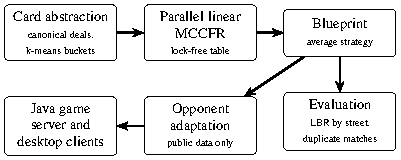
\includegraphics[width=\columnwidth]{figures/system.pdf}
\caption{The system. A Rust trainer builds the card abstraction and the blueprint; the
evaluation tools measure it; the adaptation layer and the Java server bring it to the table.}
\label{fig:system}
\end{figure}

Fig.~\ref{fig:system} shows the system. This section describes the trainer.

\subsection{Betting Abstraction}
The first bet or raise of a betting round may be half the pot, the pot or twice the pot, where
``pot'' means the pot after calling; the next two raises are pot-sized; moving all-in is always
allowed; after three raises a player may only fold, call or move all-in. A player may fold only
when facing a bet. An information set consists of the full betting history and the bucket of
the player's cards on the current round. Earlier buckets are forgotten (imperfect recall), as in
Pluribus.

\subsection{Card Abstraction}
\textbf{Preflop.} The 169 strategically distinct starting hands, which loses nothing.

\textbf{Canonical deals.} A deal is renamed to the smallest of its 24 suit permutations, giving
1\,286\,792 distinct flops and 13\,960\,050 distinct turns, the published
counts~\cite{waugh2013}.

\textbf{Flop and turn.} For every canonical deal we compute a histogram of the hand's river
strength over the cards still to come: on the turn every river card is tried, on the flop 96
random run-outs; on each resulting board the strength is estimated against 64 random opponent
hands. Histograms have 16 bins and are compared by the squared distance between their cumulative
forms, which approximates earth mover's distance. k-means, started by k-means++ and run on all
cores, groups them into 200 buckets per round. Buckets are numbered from weakest to strongest
mean strength.

\textbf{River.} The exact probability of beating a random hand, over all 990 opponent hands, in
200 buckets of equal size. Both players' river strengths are computed from one set of 1\,081
hand scores per board.

Building the abstraction takes about four minutes on twelve cores; the tables occupy 137~MB.

\subsection{Parallel Linear MCCFR}
Each iteration samples one deal, then walks the tree once per player with external
sampling~\cite{lanctot2009}: the updated player tries every action, the opponent samples one
from its current strategy, and regret matching gives the current strategy at every information
set. All threads share one open-addressing hash table of information sets and update it without
locks; occasional lost updates add little to the sampling noise~\cite{recht2011}. Linear
weighting is applied as in Pluribus: training runs in epochs of $10^5$ iterations and after
epoch $e$ every regret and strategy sum is multiplied by $e/(e+1)$.

Regrets and strategy sums are stored as 64-bit floats. With 32-bit floats the sums at the busiest
preflop nodes reached tens of millions after a few million iterations, where an update of about
one is lost to rounding and training quietly stalls.

\subsection{River Re-solving}
When the river card is dealt, the agent stops playing its river buckets and solves the rest of
the hand. The subgame starts at the river with the actual pot and uses the blueprint's bet
sizes. Each player's range is the product, over that player's earlier actions, of the
probability that the blueprint takes the action with each pair of hole cards; the ranges use no
private cards. The opponent's probabilities are floored at 0.01 per action, so that a range
never collapses after an action the blueprint rarely takes. This is unsafe
re-solving~\cite{brown2018}: it trusts the opponent's range.

The subgame is solved by discounted CFR~\cite{brown2019dcfr} ($\alpha=1.5$, $\beta=0$,
$\gamma=2$) in vector form: every decision keeps regrets for each of the up to 1\,081 hands
that miss the board, and both players are updated in turn. A fold is valued for all hands at
once from the total opponent weight minus the weight on hands that share a card. A showdown is
valued by sweeping the hands in order of strength while keeping running totals per card, so
that card removal is exact and the cost is linear in the number of hands. Hands with negligible
weight in both ranges are left out. On a river with 117 subgame nodes and full ranges, 200
iterations take about 0.3~s on one core and leave an exploitability of 0.025 big blinds.

\begin{table}[t]
\caption{Training Speed on an Apple M3 Pro (12 Cores), Heads-Up NLHE, 50 Buckets per Round}
\label{tab:speed}
\centering
\begin{tabular}{lrr}
\hline
Change & 1 core & 12 cores \\
 & \multicolumn{2}{c}{(iterations per second)} \\
\hline
First implementation & 4\,100 & -- \\
Fixed-size states and action lists; shared table & 5\,430 & 46\,517 \\
One deal shared by both players' walks & 10\,000 & 84\,021 \\
River strengths of both players from one scoring & 23\,265 & 199\,067 \\
\hline
\end{tabular}
\end{table}

Table~\ref{tab:speed} shows how speed developed. Sixty million iterations of a 200-bucket
abstraction, about 3.08 million information sets, take seven minutes.

% ============================================================================
\section{Evaluation Methodology}
\label{sec:evaluation}

\subsection{Duplicate Matches}
Two strategies play every deal twice with seats exchanged, so neither profits from better cards.
We report the mean and a 95\% interval of $\pm1.96$ standard errors of the per-deal result.

\subsection{Local Best Response by Betting Round}
Our LBR follows~\cite{lisy2017}. It keeps a weight for each of the 1\,326 hands the strategy may
hold and, after every action of the strategy, multiplies each weight by the probability that the
strategy takes that action with that hand. At its own decision it values folding at zero,
checking or calling an amount $c$ into a pot $P$ at $W(P+c)-c$, where $W$ is its probability of
winning against the weighted range, and a bet that adds $d$ chips at
\begin{equation}
F P + (1-F)\big(W'(P+2d-c)-d\big),
\label{eq:lbr}
\end{equation}
where $F$ is the probability that the strategy folds and $W'$ the winning probability against
the hands that do not fold. LBR uses the strategy's own bet sizes. Winning probabilities are
exact on the river and the turn and sampled on earlier rounds.

LBR's check-down valuation plays the preflop badly: allowed to deviate there, it loses money and
hides later leaks. By default it therefore plays the strategy itself before the flop. To locate
leaks we also let it deviate on \emph{one} round only and play the strategy everywhere else;
since the strategy against itself breaks even, what LBR then wins is what that round alone
gives away.

\subsection{A Pitfall in Seeding Parallel Generators}
A first version seeded each thread's generator with \texttt{seed XOR (index $\times$ step)},
where \texttt{step} is the constant that SplitMix64~\cite{steele2014} adds to its state on every
draw. For small seeds the resulting states differ by small multiples of \texttt{step}, so some
threads' streams were exact copies of others shifted by a few draws, and they dealt nearly the
same hands. The number of independent hands was much smaller than reported, margins were
understated, and an LBR that never deviates appeared to win $17.7\pm4.6~\bbh$ across eight
seeds. Hashing seed and index together before seeding removes the overlap; the same check then
gives values scattered around zero (mean $-2.4$, each $\pm36$). We keep it as a test, together
with a test that neighbouring streams never repeat each other's output. Results in this article
use the corrected generator.

% ============================================================================
\section{Opponent Adaptation}
\label{sec:adaptation}
The adaptation layer was first built on a simulation-based base agent, described here; placing it
on the blueprint is in progress (Section~\ref{sec:results-adaptation}).

\subsection{Base Agent}
Before the flop the base agent opens a share of hands that widens toward the button, from 15\%
in the earliest seat to 45\% on the button. After the flop it estimates its equity by dealing the
unseen cards 600 times (800 for the adaptive agent) against a range for each opponent, defined by
a width and a connectedness set from the opponent's actions in the hand. It bets for value when
its equity $e$ exceeds $0.2 + 0.8/(n+1)$ for $n$ opponents and calls when $e \ge c/(P+c) + m$,
with margin $m = 0.04$ on the river and $0.08$ otherwise, plus $0.05$ after a raise.

\subsection{Opponent Book}
For each opponent the agent counts, across all observed hands, voluntary entries, preflop
raises, folds to preflop raises and to postflop bets, postflop aggression, and, when cards are
shown after postflop betting, how many such hands were weak (strength below 0.45). Each rate is
shrunk toward a typical player's value $p_0$:
\begin{equation}
\hat{p} = \frac{w\,p_0 + k}{w + N},
\label{eq:shrink}
\end{equation}
where $k$ counts occurrences in $N$ opportunities, with $w=12$ before the flop, $8$ after it and
$4$ for the bluff rate.

\subsection{Bounded Adjustments}
Five judgments change with the estimates, each within a fixed cap: the opponent's range (width
$\times0.4$ to $\times2.5$, connectedness $\times0.35$ to $\times1.3$), bluffing (at most 65\%
of eligible spots, never into three or more players), value betting (bar $\pm0.08$, size 0.4 to
1.1 pots), calling (margin $-0.07$ to $+0.08$) and opening (share $\times0.8$ to $\times1.5$).
A bet of $b$ pots breaks even as a bluff when all opponents fold with probability $b/(1+b)$; with
$F$ the product of their fold-to-bet estimates, the agent bluffs a weak hand with probability
\begin{equation}
\min\!\Big(0.65,\; s\,\big(0.15 + 2.5\,(F - \tfrac{b}{1+b} - 0.04)\big)\Big),
\label{eq:bluff}
\end{equation}
when the bracket is positive, with $b=0.7$ and $s$ equal to 0.55, 0.8 and 1 on the flop, turn
and river. When every estimate equals the typical player the agent plays exactly as the base
agent; a test confirms identical decisions in 400 random situations.

% ============================================================================
\section{Experiments}
\label{sec:results}

\subsection{Solver Validation}
Table~\ref{tab:validation} lists the checks against published values, and Fig.~\ref{fig:leduc}
shows convergence on Leduc Hold'em. On this small game, walking the whole tree with CFR+ or
discounted CFR is fastest; sampling pays off only in games too large to walk.

\begin{table}[t]
\caption{Checks Against Published Values}
\label{tab:validation}
\centering
\begin{tabular}{lrr}
\hline
Quantity & Ours & Published \\
\hline
Five-card hands per category & match & standard \\
Seven-card hands per category & match & standard \\
Canonical flops & 1\,286\,792 & 1\,286\,792~\cite{waugh2013} \\
Canonical turns & 13\,960\,050 & 13\,960\,050~\cite{waugh2013} \\
Kuhn, uniform play: exploitability & 0.458333 & 0.458333 \\
Leduc, uniform play: exploitability & 2.373611 & 2.373611 \\
Kuhn: first player's value & $-0.05556$ & $-1/18$ \\
Leduc: first player's value & $-0.0856$ & $-0.0856$ \\
\hline
\multicolumn{3}{p{0.92\columnwidth}}{\footnotesize Hand counts: all 2\,598\,960 five-card and
133\,784\,560 seven-card hands. Uniform-play values are half of OpenSpiel's NashConv.}
\end{tabular}
\end{table}

\begin{figure}[t]
\centering
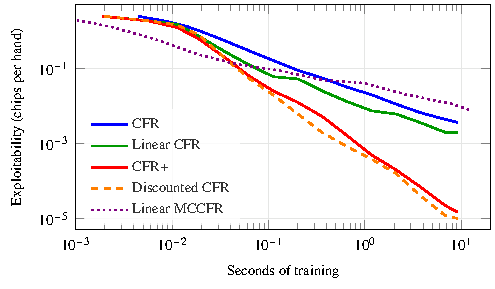
\includegraphics[width=\columnwidth]{figures/leduc.pdf}
\caption{Exploitability of each solver's average strategy on Leduc Hold'em against training time
on one core. Exploitability is computed exactly by best response.}
\label{fig:leduc}
\end{figure}

\subsection{Where the Blueprint Leaks}
Table~\ref{tab:streets} and Fig.~\ref{fig:streets} give LBR results for blueprints trained on
the 200-bucket abstraction for two, twenty and sixty million iterations. Each value uses 100\,000
deals (200\,000 hands).

\begin{table}[t]
\caption{LBR Winnings (\mbb) Against the Blueprint, by the Round on Which LBR May Deviate}
\label{tab:streets}
\centering
\begin{tabular}{lrrrrr}
\hline
Iterations & Flop & Turn & River & Postflop & Margin \\
\hline
$2\times10^6$ & $-109$ & 91 & 276 & 479 & $\pm75$ \\
$2\times10^7$ & $-10$ & 220 & 586 & 635 & $\pm75$ \\
$6\times10^7$ & $-9$ & 190 & 736 & 793 & $\pm75$ \\
\hline
\multicolumn{6}{p{0.9\columnwidth}}{\footnotesize ``Postflop'' lets LBR deviate on the flop,
turn and river. Margins are the largest 95\% interval in each row.}
\end{tabular}
\end{table}

\begin{figure}[t]
\centering
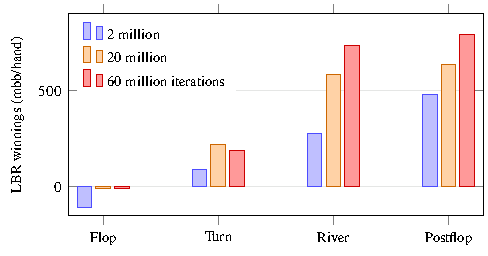
\includegraphics[width=\columnwidth]{figures/streets.pdf}
\caption{What each betting round gives away. LBR deviates only on the round named (or on all
three after the flop) and plays the blueprint elsewhere. The river leak grows with training.}
\label{fig:streets}
\end{figure}

The flop is close to unexploitable at every length. The turn leaks moderately. The river leaks
most, and more the longer the strategy trains. Yet training is not failing: in the same
abstraction family, a 20-million-iteration strategy beats a 2-million one head to head by
$18.5\pm3.6$ and $13.5\pm3.6~\bbh$ (two seeds) and a 200\,000 one by $68.1\pm5.0~\bbh$, over
400\,000 hands each\footnote{These matches used the earlier 50-bucket abstraction.}. Training
sharpens play within the river buckets, and an opponent with exact cards punishes the
distinctions those buckets cannot draw: a river bucket measures strength against a random hand,
which says little about strength against the narrow range an opponent holds after three rounds
of betting. This matches the overfitting described in~\cite{johanson2013} and locates it.

\subsection{Fixing the River}
Richer buckets were tried first. With opponent cluster hand strength~\cite{johanson2013}, a
river hand is described by its probability of beating each of eight clusters of starting hands,
and k-means on these vectors gives 200 buckets (flop and turn unchanged). River-only LBR was
359, 635 and 695~\mbb{} at the three training lengths, no different from Table~\ref{tab:streets}
within the margins, and still rising with training. The leak does not come from what a bucket
knows, but from bucketing itself: every hand in a bucket must play alike, and an opponent with
exact cards reads the lines training draws between buckets.

Re-solving removes it (Table~\ref{tab:resolve}). LBR that may deviate only on the river wins
nothing measurable, and exploitability after the flop falls by 70\% for the longer-trained
blueprint. With re-solving, longer training no longer hurts. The remaining exploitability is
mostly on the turn.

\begin{table}[t]
\caption{LBR Winnings (\mbb) With River Buckets and With River Re-solving}
\label{tab:resolve}
\centering
\begin{tabular}{lrrrr}
\hline
 & \multicolumn{2}{c}{River only} & \multicolumn{2}{c}{Postflop} \\
Iterations & Buckets & Re-solved & Buckets & Re-solved \\
\hline
$2\times10^6$ & $276\pm67$ & $-59\pm90$ & $479\pm75$ & $275\pm103$ \\
$6\times10^7$ & $736\pm57$ & $7\pm64$ & $793\pm75$ & $243\pm97$ \\
\hline
\multicolumn{5}{p{0.9\columnwidth}}{\footnotesize 200 histogram buckets; re-solving with 200
iterations; 100\,000 hands per value.}
\end{tabular}
\end{table}

\subsection{Opponent Adaptation}
\label{sec:results-adaptation}
Table~\ref{tab:adapt} reports heads-up matches of the simulation-based base agent and its
adaptive version against six opponents: two rule-based agents (Easy, Solid) and four with
deliberate flaws (Caller never folds; Maniac bets or raises 65\% of the time; Over-folder folds
to any postflop bet without a strong hand; Chameleon alternates between over-folding and calling
every 1\,500 decisions, to punish an agent that adapts).

\begin{table}[t]
\caption{Heads-Up Win Rates (\bbh, 95\% Intervals) of the Base and Adaptive Agents}
\label{tab:adapt}
\centering
\begin{tabular}{lrrr}
\hline
Opponent & Hands & Base agent & Adaptive agent \\
\hline
Caller & 200\,000 & $345.0\pm5.4$ & $1079.4\pm15.4$ \\
Maniac & 200\,000 & $292.8\pm11.0$ & $562.8\pm15.2$ \\
Chameleon & 200\,000 & $105.2\pm2.8$ & $233.8\pm6.4$ \\
Over-folder & 200\,000 & $41.4\pm1.3$ & $65.5\pm1.3$ \\
Solid & 300\,000 & $35.5\pm1.7$ & $57.1\pm1.6$ \\
Easy & 300\,000 & $28.9\pm2.3$ & $42.1\pm2.5$ \\
\hline
\end{tabular}
\end{table}

The adaptive agent wins more than the base agent against every opponent with no overlap between
intervals, more than doubles its win rate against Chameleon, and beats the base agent directly by
$8.4\pm3.4~\bbh$ over 200\,000 hands. At a six-player table of sound agents the advantage is
small (adaptive $+7.8$ and $+3.9$, base $-2.1$ and $-3.8$, $\pm2.9$, over 600\,000 hands).

\pending{The same layer on the blueprint: win rates against the six opponents, and its own LBR
exploitability compared with the blueprint's, to show what adaptation costs in safety.}

\pending{Ablations: each of the five adjustments switched off in turn; learning curves of the
gain against hands observed.}

% ============================================================================
\section{Limitations}
\label{sec:limits}
\textbf{Unsafe re-solving.} The river solver trusts the opponent's range as the blueprint
implies it. An opponent who plays differently before the river can make that range wrong; safe
re-solving~\cite{brown2018} would bound the damage. LBR after the flop does deviate before the
river, and the result still improved, but this is not a guarantee.

\textbf{LBR is a lower bound.} It uses the strategy's own bet sizes and a check-down valuation;
a full best response would win more.

\textbf{Abstraction.} The river leak shows the limits of strength-against-random buckets; all
results are for one betting abstraction.

\textbf{Synthetic opponents.} All opponents in Table~\ref{tab:adapt} were written by us, and four
are extreme by design. Gains against people will be smaller. Chameleon tests one switching
pattern, not an adversary that models our agent.

\textbf{Informal safety.} The caps bound how far the adaptive agent moves, not its
exploitability; a restricted Nash response~\cite{johanson2008} on top of the blueprint would give
a formal bound.

\textbf{No external benchmark or human study yet.} \pending{Matches against Slumbot; a study with
human players.}

% ============================================================================
\section{Conclusion}
\label{sec:conclusion}
A consumer laptop trains a heads-up NLHE blueprint at about $2\times10^5$ iterations per second.
Restricting local best response to one betting round turns a single exploitability number into a
map of where a strategy is weak; for our strategies the map points at the river, whose leak grows
as the strategy overfits its card abstraction. Richer buckets do not remove it; solving the river
hand by hand during play does, and cuts exploitability after the flop by 70\%. Careful seeding of parallel generators matters as
much as the solver for trustworthy measurements. A bounded opponent model built from public
information raises win rates against every opponent type tested, including one built to punish
it. Next steps are re-solving from the turn, moving the adaptation layer onto the blueprint as
a restricted Nash response, and external benchmarks.

\section*{Data and Code Availability}
The game engine, server, solvers and evaluation tools, with the commands and seeds behind every
result, are available at \pending{https://github.com/SakD2006/holdem (to be made public, with a
fixed release)}.

\section*{Acknowledgment}
The author used Claude (Anthropic), an AI assistant, to help write and review the software
described here and to draft and edit the text of all sections of this article. The author
designed the study, ran the experiments, checked every result and reference, and takes
responsibility for the content. \pending{Adjust this statement to match actual use; add anyone
who helped but is not an author.}

% ============================================================================
\begin{thebibliography}{00}
% Every entry is to be checked against the published version before submission.

\bibitem{brown2018} N. Brown and T. Sandholm, ``Superhuman AI for heads-up no-limit poker:
Libratus beats top professionals,'' \emph{Science}, vol. 359, no. 6374, pp. 418--424, 2018.

\bibitem{brown2019} N. Brown and T. Sandholm, ``Superhuman AI for multiplayer poker,''
\emph{Science}, vol. 365, no. 6456, pp. 885--890, 2019.

\bibitem{lisy2017} V. Lis\'{y} and M. Bowling, ``Equilibrium approximation quality of current
no-limit poker bots,'' in \emph{Proc. AAAI Workshop Comput. Poker Imperfect Inf. Games}, 2017.

\bibitem{waugh2009} K. Waugh, D. Schnizlein, M. Bowling, and D. Szafron, ``Abstraction
pathologies in extensive games,'' in \emph{Proc. 8th Int. Conf. Auton. Agents Multiagent Syst.
(AAMAS)}, 2009, pp. 781--788.

\bibitem{johanson2013} M. Johanson, N. Burch, R. Valenzano, and M. Bowling, ``Evaluating
state-space abstractions in extensive-form games,'' in \emph{Proc. 12th Int. Conf. Auton. Agents
Multiagent Syst. (AAMAS)}, 2013, pp. 271--278.

\bibitem{zinkevich2007} M. Zinkevich, M. Johanson, M. Bowling, and C. Piccione, ``Regret
minimization in games with incomplete information,'' in \emph{Adv. Neural Inf. Process. Syst.},
vol. 20, 2008, pp. 1729--1736.

\bibitem{tammelin2014} O. Tammelin, ``Solving large imperfect information games using CFR+,''
2014, \emph{arXiv:1407.5042}.

\bibitem{brown2019dcfr} N. Brown and T. Sandholm, ``Solving imperfect-information games via
discounted regret minimization,'' in \emph{Proc. AAAI Conf. Artif. Intell.}, vol. 33, 2019,
pp. 1829--1836.

\bibitem{lanctot2009} M. Lanctot, K. Waugh, M. Zinkevich, and M. Bowling, ``Monte Carlo sampling
for regret minimization in extensive games,'' in \emph{Adv. Neural Inf. Process. Syst.}, vol. 22,
2009, pp. 1078--1086.

\bibitem{moravcik2017} M. Morav\v{c}\'{i}k \emph{et al.}, ``DeepStack: Expert-level artificial
intelligence in heads-up no-limit poker,'' \emph{Science}, vol. 356, no. 6337, pp. 508--513,
2017.

\bibitem{brown2020} N. Brown, A. Bakhtin, A. Lerer, and Q. Gong, ``Combining deep reinforcement
learning and search for imperfect-information games,'' in \emph{Adv. Neural Inf. Process. Syst.},
vol. 33, 2020, pp. 17057--17069.

\bibitem{waugh2013} K. Waugh, ``A fast and optimal hand isomorphism algorithm,'' in \emph{Proc.
AAAI Workshop Comput. Poker Imperfect Inf.}, 2013.

\bibitem{billings1998} D. Billings, D. Papp, J. Schaeffer, and D. Szafron, ``Opponent modeling
in poker,'' in \emph{Proc. 15th Nat. Conf. Artif. Intell. (AAAI)}, 1998, pp. 493--499.

\bibitem{billings2002} D. Billings, A. Davidson, J. Schaeffer, and D. Szafron, ``The challenge
of poker,'' \emph{Artif. Intell.}, vol. 134, nos. 1--2, pp. 201--240, 2002.

\bibitem{southey2005} F. Southey \emph{et al.}, ``Bayes' bluff: Opponent modelling in poker,''
in \emph{Proc. 21st Conf. Uncertainty Artif. Intell. (UAI)}, 2005, pp. 550--558.

\bibitem{johanson2008} M. Johanson, M. Zinkevich, and M. Bowling, ``Computing robust
counter-strategies,'' in \emph{Adv. Neural Inf. Process. Syst.}, vol. 20, 2008, pp. 721--728.

\bibitem{ganzfried2011} S. Ganzfried and T. Sandholm, ``Game theory-based opponent modeling in
large imperfect-information games,'' in \emph{Proc. 10th Int. Conf. Auton. Agents Multiagent
Syst. (AAMAS)}, 2011, pp. 533--540.

\bibitem{ganzfried2015} S. Ganzfried and T. Sandholm, ``Safe opponent exploitation,'' \emph{ACM
Trans. Econ. Comput.}, vol. 3, no. 2, Art. no. 8, 2015.

\bibitem{recht2011} B. Recht, C. R\'{e}, S. Wright, and F. Niu, ``Hogwild!: A lock-free approach
to parallelizing stochastic gradient descent,'' in \emph{Adv. Neural Inf. Process. Syst.},
vol. 24, 2011, pp. 693--701.

\bibitem{steele2014} G. L. Steele, Jr., D. Lea, and C. H. Flood, ``Fast splittable pseudorandom
number generators,'' in \emph{Proc. ACM Int. Conf. Object Oriented Program. Syst. Lang. Appl.
(OOPSLA)}, 2014, pp. 453--472.

\end{thebibliography}

% ============================================================================
\begin{IEEEbiography}[{\fbox{\parbox[c][1.2in][c]{0.95in}{\centering\scriptsize Author\\photo}}}]{Saksham Dubey}
\pending{is pursuing the B.Tech. degree in [branch] at the School of Computer Science and
Engineering, Vellore Institute of Technology, Vellore, India, since 2024. His research interests
include game-playing artificial intelligence, imperfect-information games and systems
programming.}
\end{IEEEbiography}

\EOD

\end{document}
